\documentclass[11pt,a4paper]{article}
\usepackage[utf8]{inputenc}
\usepackage[T1]{fontenc}
\usepackage[indonesian]{babel}
\usepackage{geometry}
\usepackage{titlesec}
\usepackage{enumitem}
\usepackage{booktabs}
\usepackage{longtable}
\usepackage{graphicx}
\usepackage{hyperref}
\usepackage{array}
\usepackage{caption}
\usepackage{lipsum} % Hapus jika tidak diperlukan
\usepackage{rotating}  % Pastikan sudah ada di preamble
\usepackage{array}     % Untuk kontrol kolom lebih presisi

% Margin
\geometry{left=3cm,right=2.5cm,top=2.5cm,bottom=2.5cm}

% Judul bagian
\titleformat{\section}{\large\bfseries\centering}{\thesection}{1em}{}
\titleformat{\subsection}{\normalsize\bfseries}{\thesubsection}{1em}{}

% Spasi paragraf
\setlength{\parindent}{1.5em}
\setlength{\parskip}{0.5em}

% Hyperlink settings
\hypersetup{
    colorlinks=true,
    linkcolor=black,
    filecolor=magenta,      
    urlcolor=cyan,
    pdftitle={Roadmap Pusat Riset IoT: Mewujudkan Ekosistem Cerdas yang Berkeadilan (2025–2045)},
    pdfauthor={Tim Riset IoT},
}

% ====== FOOTER: Dokumen Pusat Riset IoT Polinema 2025 - Roadmap Penelitian - hal xx dari yy ======
\usepackage{fancyhdr}
\usepackage{lastpage} % Untuk mendapatkan total halaman (yy)

% Atur gaya halaman
\pagestyle{fancy}
\fancyhf{} % Hapus header/footer default
\lfoot{\small{Dokumen Pusat Riset IoT Polinema 2025 \quad Roadmap Penelitian \quad hal \thepage\ dari \pageref{LastPage}}}
\renewcommand{\headrulewidth}{0pt} % Hilangkan garis header
\renewcommand{\footrulewidth}{0.4pt} % Tambahkan garis tipis di bawah footer (opsional)
\fancyfootoffset{0pt} % Pastikan footer tidak terpotong oleh margin

% Pastikan halaman pertama juga punya footer (biasanya style plain tidak punya)
\fancypagestyle{plain}{
    \fancyhf{}
    \lfoot{\small{Dokumen Pusat Riset IoT Polinema, 2025 \quad Roadmap Penelitian \quad hal \thepage\ dari \pageref{LastPage}}}
    \renewcommand{\footrulewidth}{0.4pt}
}

\newenvironment{vision}{%
  \begin{list}{}{%
    \setlength{\leftmargin}{1cm}%
    \setlength{\rightmargin}{1cm}%
    \setlength{\topsep}{1em}%
    \setlength{\partopsep}{0pt}%
    \setlength{\parsep}{0pt}%
    \setlength{\itemsep}{0pt}%
  }%
  \item\small
  % \itshape
}{%
  \end{list}%
}

% Judul Dokumen
\title{\textbf{Roadmap Pusat Riset IoT \\ Mewujudkan Ekosistem Cerdas yang Berdampak \\ (2025–2045)}}
\author{Tim Pusat Riset IoT \\ [0.5em] \small Politeknik Negeri Malang}
\date{\today}

\begin{document}

\maketitle

% \begin{center}
% \textbf{\large Visi} \\
% \vspace{0.5em}
%     \textit{“Mewujudkan Ekosistem Cerdas yang Berdampak”, pusat riset IoT ini berkomitmen untuk tidak hanya menciptakan teknologi yang cerdas, tetapi juga secara nyata memberikan solusi terukur terhadap tantangan strategis nasional di bidang pendidikan, kesehatan, lingkungan, dan tata kelola kampus — sejalan dengan prioritas Kemendikbudristek dalam mendorong transformasi digital berbasis riset terapan, inovasi berkelanjutan, dan kontribusi langsung terhadap pembangunan sumber daya manusia unggul. Dengan membangun infrastruktur C-IoT-TB sebagai laboratorium hidup, riset ini menekankan pada impact-driven innovation: setiap sensor, algoritma, atau sistem yang dikembangkan harus mampu membuktikan manfaatnya bagi masyarakat, meningkatkan efisiensi layanan publik, serta menjadi model replikabel bagi perguruan tinggi lain di Indonesia. Dengan demikian, keberhasilan tidak dinilai dari jumlah publikasi semata, tetapi dari seberapa jauh teknologi yang dihasilkan mampu mengubah praktik nyata, memperkuat ketahanan sosial-ekologis, dan menjadi tulang punggung ekosistem riset berdampak yang diamanatkan dalam Rencana Strategis Kemendikbudristek 2025–2045."}
% \end{center}

\begin{vision}
    \begin{center}
        \textbf{\large Visi} \\
        \vspace{0.5em}
    \end{center}
    \begin{center}
        \textbf{Mewujudkan Ekosistem Cerdas yang Berdampak}\\
    \end{center}
    Pusat riset IoT ini berkomitmen untuk tidak hanya menciptakan teknologi yang cerdas, tetapi juga secara nyata memberikan solusi terukur terhadap tantangan strategis nasional di bidang pendidikan, kesehatan, lingkungan, dan tata kelola kampus — sejalan dengan prioritas Kemendikbudristek dalam mendorong transformasi digital berbasis riset terapan, inovasi berkelanjutan, dan kontribusi langsung terhadap pembangunan sumber daya manusia unggul. Dengan membangun infrastruktur C-IoT-TB sebagai laboratorium hidup, riset ini menekankan pada impact-driven innovation: setiap sensor, algoritma, atau sistem yang dikembangkan harus mampu membuktikan manfaatnya bagi masyarakat, meningkatkan efisiensi layanan publik, serta menjadi model replikabel bagi perguruan tinggi lain di Indonesia. Dengan demikian, keberhasilan tidak dinilai dari jumlah publikasi semata, tetapi dari seberapa jauh teknologi yang dihasilkan mampu mengubah praktik nyata, memperkuat ketahanan sosial-ekologis, dan menjadi tulang punggung ekosistem riset berdampak yang diamanatkan dalam Rencana Strategis Kemendikbudristek 2025–2045
\end{vision}

% --- PERNYATAAN MISI ---
% \begin{center}
% \textbf{\large Misi Pusat Riset IoT} \\
% \vspace{0.5em}
% \small
% \textit{“Mengembangkan infrastruktur IoT terbuka (C-IoT-TB) sebagai laboratorium hidup untuk penelitian terapan di bidang kesehatan, lingkungan, dan smart campus, dengan pendekatan kolaboratif, rendah biaya, dan berkeadilan multidimensi — memastikan bahwa teknologi IoT tidak hanya cerdas, tetapi juga inklusif, transparan, dan memberdayakan bagi semua kelompok masyarakat, terutama yang rentan dan terpinggirkan.”}
% \end{center}
\begin{vision}
    \begin{center}
        \textbf{\large Misi} \\
        \vspace{0.5em}
    \end{center}
    Mengembangkan infrastruktur IoT terbuka (C-IoT-TB) sebagai laboratorium hidup untuk penelitian terapan di bidang kesehatan, lingkungan, dan smart campus, dengan pendekatan kolaboratif, rendah biaya, dan berkeadilan multidimensi — memastikan bahwa teknologi IoT tidak hanya cerdas, tetapi juga inklusif, transparan, dan memberdayakan bagi semua kelompok masyarakat, terutama yang rentan dan terpinggirkan
\end{vision}




% % --- VISI GLOBAL ---
% \begin{center}
% \textbf{\large Visi} \\
% \vspace{0.5em}
% \small
% \textit{“Menciptakan ekosistem cerdas yang terhubung secara seamless, aman, dan adil untuk meningkatkan kesejahteraan manusia, keberlanjutan lingkungan, dan ketahanan sosial di tingkat nasional dan global.”}
% \end{center}

\begin{abstract}
    Dokumen ini menyajikan roadmap strategis 15 tahun bagi pusat riset IoT yang baru dibentuk pada tahun 2025, dengan sumber daya manusia terbatas, pengetahuan teknis awal minimal, dan tanpa infrastruktur eksisting. Meskipun demikian, grup ini memiliki visi ambisius: \textit{“To pioneer an intelligent, interconnected ecosystem that enhances human well-being, sustainability, and resilience across health, home, city, industry, and environment — empowering lives through seamless, secure, and equitable IoT innovation.”}

    Roadmap ini dirancang secara realistis dan bertahap, mengintegrasikan prinsip \textit{“Start Small, Think Big”} dan \textit{“Technology for Justice”}. Lima tahap utama — mulai dari pembangunan infrastruktur dasar \textbf{C-IoT-TB (Campus-based IoT Testbed)} hingga pencapaian pengaruh global — disusun dengan aktivitas operasional, pengembangan kapasitas SDM, dan indikator keberhasilan terukur (KPI). Setiap tahap menekankan aspek keadilan multidimensi: akses, partisipasi, distribusi, proses, representasi, dan keberlanjutan lingkungan.

    Dokumen ini berfungsi sebagai panduan operasional, alat evaluasi internal, serta dasar permohonan hibah riset nasional dan internasional. Dengan pendekatan ini, grup tidak hanya membangun teknologi, tetapi juga membangun keadilan sosial melalui inovasi.
\end{abstract}

\tableofcontents
\newpage

\section{Ruang Lingkup Bidang Riset}
\subsection{Dasar dan Arah Strategis}
\begin{enumerate}
    \item Visi, misi, tujuan pusat riset IoT.
    \item Tren global dan nasional IoT (industri 4.0, smart city, smart agriculture, dsb).
    \item Kebijakan nasional (Making Indonesia 4.0, RIRN/RIP, SN-Dikti, RIRN bidang TIK).
    \item Bidang prioritas riset: industri, kesehatan, pendidikan, transportasi, energi, pertanian, pertahanan.
\end{enumerate}
\subsection{Bidang-bidang Penelitian Utama}
\begin{enumerate}
    \item \textbf{Perangkat IoT (Hardware \& Sensor)}: Embedded system, microcontroller, sensor network.
    \item \textbf{Konektivitas \& Infrastruktur}: Lorawan, MQTT, LPWAN, 5G, edge computing, cloud integration.
    \item \textbf{Platform \& Middleware}: Sistem operasi IoT, interoperability, API, middleware untuk integrasi.
    \item \textbf{Keamanan \& Privasi}: IoT security, cryptography, identity management.
    \item \textbf{Analitik \& AI}: Big data IoT, machine learning, predictive analytics.
    \item \textbf{Aplikasi Vertikal}: Smart city, smart home, smart agriculture, healthtech, industrial IoT, Smart IoT Ecosystems.
\end{enumerate}



\section{Pendahuluan}

Pusat riset IoT ini didirikan pada tahun 2023 dalam kondisi awal yang sangat terbatas: jumlah anggota sedikit, minim pengalaman teknis IoT, tidak ada perangkat atau infrastruktur eksisting, serta belum ada rekam jejak publikasi. Namun, visi jangka panjangnya jelas dan ambisius — menciptakan ekosistem cerdas yang meningkatkan kesejahteraan manusia, keberlanjutan lingkungan, dan ketahanan sosial.

Untuk menjembatani kesenjangan antara visi besar dan realitas awal, roadmap ini mengadopsi dua prinsip inti:
\begin{enumerate}[leftmargin=*]
    \item \textbf{Start Small, Think Big}: Memulai dari skala mikro (satu ruangan, satu sensor, satu masalah nyata) untuk membangun bukti konsep yang meyakinkan.
    \item \textbf{Technology for Justice}: Teknologi IoT tidak boleh memperdalam ketidaksetaraan — ia harus menjadi alat pemberdayaan bagi kelompok rentan, termasuk lansia, penyandang disabilitas, mahasiswa kurang mampu, dan komunitas pinggiran.
\end{enumerate}

Infrastruktur awal \textbf{Pembangunan Infrastruktur IoT Campus Testbed (C-IoT-TB) untuk Penelitian Jaringan Sensor Nirkabel dan Aplikasi IoT Terapan} menjadi fondasi teknis utama pada Tahap 1. Namun, keberhasilannya tidak diukur hanya oleh jumlah node atau koneksi, tetapi oleh sejauh mana ia mampu menjadi \textit{platform inklusif} — tempat semua orang, terlepas dari latar belakangnya, dapat berpartisipasi, belajar, dan mendapatkan manfaat.

Roadmap ini terbagi menjadi lima periode strategis selama 20 tahun (2025–2045), masing-masing dengan fokus spesifik, aktivitas terstruktur, pengembangan SDM, dan indikator keberhasilan terukur. Setiap tahap dirancang untuk membangun kapasitas secara bertahap, sekaligus memperdalam komitmen terhadap keadilan sosial dan keberlanjutan.

\section{Tahap 1: Pembangunan Fondasi (2025–2029)}
\label{sec:tahap1}

\textbf{Fokus:} Membangun kapasitas dasar, infrastruktur awal, dan budaya riset.\\
\textbf{Visi Sementara:} \textit{From Zero to First Prototype}

\begin{itemize}
    \item \textbf{Aktivitas Inti:}
          \begin{enumerate}
              \item Bangun \textbf{C-IoT-TB v1.0}: 50 node sensor (suhu, kelembapan, gerak, kualitas udara) di area kampus terbatas.
              \item Gunakan teknologi \textbf{LoRaWAN} dan \textbf{NB-IoT} untuk komunikasi nirkabel hemat energi.
              \item Bangun gateway lokal (RAKwireless RAK7249 / RAK7258, senseCAP gateway)+ server edge (Raspberry Pi, Jetson) + database sederhana (InfluxDB + Grafana).
              \item Gunakan jaringan internet kampus; tidak perlu infrastruktur khusus.
          \end{enumerate}

    \item \textbf{Pengembangan SDM:}
          \begin{enumerate}
              \item Workshop bulanan: “IoT for Beginners” (Arduino, Python, MQTT, sensor dasar).
              \item Setiap anggota dianjurkan menyelesaikan 1 sertifikasi online (Coursera/edX: \textit{IoT Fundamentals}), dibiayai.
              \item Kolaborasi magang dengan industri lokal: 2–3 mahasiswa/tahun.
          \end{enumerate}

    \item \textbf{Proyek Mini Riset:}
          \begin{enumerate}
              \item Mahasiswa S1/S2 membuat proyek berbasis C-IoT-TB: monitoring ruang lab, deteksi kebocoran air, pengingat listrik, dll.
          \end{enumerate}
\end{itemize}

\begin{center}
    \begin{tabular}{ll}
        \toprule
        \textbf{Indikator Keberhasilan}                 & \textbf{Target (Tahun 2029)} \\
        \midrule
        Jumlah node aktif di C-IoT-TB                   & $\geq$ 50                    \\
        Jumlah proyek riset mahasiswa berbasis C-IoT-TB & $\geq$ 10                    \\
        Jumlah anggota grup bersertifikasi IoT dasar    & $\geq$ 80\%                  \\
        Publikasi ilmiah (jurnal nasional/lokakarya)    & $\geq$ 5 artikel             \\
        Kemitraan dengan 1 industri/instansi pemerintah & Ada                          \\
        Akses stabil ke data real-time dari C-IoT-TB    & 95\% uptime                  \\
        \bottomrule
    \end{tabular}
\end{center}

\textbf{Target Akhir:} Grup dikenal di lingkungan kampus sebagai “tempat belajar IoT praktis”.

\section{Tahap 2: Ekspansi dan Spesialisasi (2030–2034)}
\label{sec:tahap2}

\textbf{Fokus:} Memperdalam teknologi, membangun komunitas, dan mulai aplikasi sektoral.\\
\textbf{Visi Sementara:} \textit{From Prototype to Sector-Specific Solutions}

\begin{itemize}
    \item \textbf{Aktivitas Inti:}
          \begin{enumerate}
              \item Ekspansi C-IoT-TB ke 3 sektor prioritas: \textbf{Health}, \textbf{Environment}, \textbf{Smart Campus}.
              \item Integrasi AI dasar: machine learning untuk prediksi pola konsumsi atau kegagalan sensor.
              \item Gunakan platform open-source: ThingsBoard, Home Assistant, AWS IoT Core.
              \item Uji coba resmi \textbf{NB-IoT} melalui kerja sama operator seluler (Telkomsel/Indosat).
          \end{enumerate}

    \item \textbf{Pengembangan SDM:}
          \begin{enumerate}
              \item 2–3 anggota menempuh PhD dalam bidang IoT/Edge AI.
              \item Program “IoT Research Fellow” untuk mahasiswa S2/S3.
              \item Organisasi workshop tahunan: \textbf{Campus IoT Day}.
          \end{enumerate}

    \item \textbf{Publikasi \& Kolaborasi:}
          \begin{enumerate}
              \item Target publikasi internasional (Scopus Q2).
              \item Ajukan hibah riset nasional (LIPI, BRIN, Kemenristekdikti).
              \item Bergabung dengan jaringan nasional IoT (Indonesia IoT Network).
          \end{enumerate}
\end{itemize}

\begin{center}
    \begin{tabular}{ll}
        \toprule
        \textbf{Indikator Keberhasilan}              & \textbf{Target (Tahun 2034)}           \\
        \midrule
        Jumlah sektor teraplikasi di C-IoT-TB        & $\geq$ 3 (health, environment, campus) \\
        Jumlah node aktif                            & $\geq$ 200                             \\
        Jumlah publikasi Scopus/Q2                   & $\geq$ 8                               \\
        Jumlah peneliti S3                           & $\geq$ 3                               \\
        Hibah riset nasional yang berhasil           & $\geq$ 2                               \\
        Kerja sama formal dengan 2 industri/instansi & Ada                                    \\
        Jumlah lulusan S2/S3 dengan fokus IoT        & $\geq$ 10                              \\
        Platform C-IoT-TB terintegrasi dengan cloud  & Ya (AWS/Azure/Google Cloud)            \\
        \bottomrule
    \end{tabular}
\end{center}

\textbf{Target Akhir:} Grup diakui sebagai \textbf{pusat unggulan riset IoT tingkat regional}.

\section{Tahap 3: Integrasi dan Dampak Sistemik (2035–2038)}
\label{sec:tahap3}

\textbf{Fokus:} Menghubungkan sektor-sektor, menciptakan sistem interkoneksi, dan dampak nyata.\\
\textbf{Visi Sementara:} \textit{From Silos to Interconnected Ecosystem}

\begin{itemize}
    \item \textbf{Aktivitas Inti:}
          \begin{enumerate}
              \item Integrasi multi-sektor di C-IoT-TB v3.0:
                    \begin{itemize}
                        \item Data kualitas udara → otomatis matikan AC jika polusi tinggi.
                        \item Data kehadiran lansia → kirim notifikasi ke keluarga jika tidak aktif >24 jam.
                        \item Data konsumsi energi → dikaitkan dengan jadwal kuliah untuk optimasi beban listrik.
                    \end{itemize}
              \item Bangun \textbf{“Smart Campus Dashboard”} terpadu.
              \item Implementasi \textbf{digital twin} sederhana (model virtual kampus sinkron dengan fisik).
          \end{enumerate}

    \item \textbf{Keamanan \& Etika IoT:}
          \begin{enumerate}
              \item Implementasi protokol keamanan: TLS, DTLS, device authentication.
              \item Studi etika IoT: privasi data lansia, bias algoritma, aksesibilitas disabilitas.
          \end{enumerate}

    \item \textbf{Pengembangan SDM:}
          \begin{enumerate}
              \item 1–2 anggota melakukan postdoc di luar negeri.
              \item Undang pakar internasional sebagai visiting professor 1x/tahun.
              \item Jadikan grup tuan rumah konferensi IoT nasional.
          \end{enumerate}
\end{itemize}

\begin{center}
    \begin{tabular}{ll}
        \toprule
        \textbf{Indikator Keberhasilan}                  & \textbf{Target (Tahun 2038)} \\
        \midrule
        Jumlah integrasi lintas-sektor di C-IoT-TB       & $\geq$ 5                     \\
        Sistem digital twin kampus (versi minimal)       & Ada                          \\
        Publikasi Q1/JCR                                 & $\geq$ 10                    \\
        Paten/software copyright                         & $\geq$ 2                     \\
        Kebijakan kampus yang diadopsi berbasis data IoT & $\geq$ 1                     \\
        Jumlah alumni yang bekerja di bidang IoT         & $\geq$ 15                    \\
        Kemitraan dengan 1 perusahaan teknologi global   & Ada                          \\
        Pendanaan riset tahunan dari luar kampus         & $\geq$ Rp 1 Miliar           \\
        \bottomrule
    \end{tabular}
\end{center}

\textbf{Target Akhir:} Grup menjadi \textbf{pemimpin nasional dalam IoT terapan multi-sektor}.

\section{Tahap 4: Inovasi Berbasis Data dan Keadilan (2039–2041)}
\label{sec:tahap4}

\textbf{Fokus:} Menggunakan data untuk inovasi sosial dan inklusif.\\
\textbf{Visi Sementara:} \textit{From Smart to Equitable \& Resilient}

\begin{itemize}
    \item \textbf{Aktivitas Inti:}
          \begin{enumerate}
              \item Aplikasi IoT untuk ketahanan sosial/lingkungan:
                    \begin{itemize}
                        \item Pemantauan banjir di permukiman sekitar kampus.
                        \item Sistem peringatan dini kebakaran hutan berbasis sensor tanah.
                        \item Pelacakan rantai pasok produk UMKM lokal.
                    \end{itemize}
              \item Desain antarmuka IoT ramah disabilitas (suara, getar, visual tinggi kontras).
              \item Platform IoT gratis untuk sekolah dasar di daerah terpencil.
          \end{enumerate}

    \item \textbf{AI + IoT (AIoT):}
          \begin{enumerate}
              \item Gunakan deep learning untuk prediksi penyakit berbasis data lingkungan + kesehatan.
              \item Model AI yang bisa dijalankan di edge device (tanpa cloud) — untuk daerah tanpa internet.
          \end{enumerate}
\end{itemize}

\begin{center}
    \begin{tabular}{ll}
        \toprule
        \textbf{Indikator Keberhasilan}                       & \textbf{Target (Tahun 2041)} \\
        \midrule
        Jumlah aplikasi IoT untuk ketahanan sosial/lingkungan & $\geq$ 3                     \\
        Jumlah masyarakat di luar kampus yang terlibat        & $\geq$ 5.000 orang           \\
        AI model IoT yang di-deploy di edge device            & $\geq$ 2                     \\
        Publikasi tentang equity \& ethics in IoT             & $\geq$ 3                     \\
        Inisiatif IoT inklusif mendapat penghargaan nasional  & Ada                          \\
        Jumlah startup spin-off dari grup                     & $\geq$ 1                     \\
        \bottomrule
    \end{tabular}
\end{center}

\textbf{Target Akhir:} Grup menjadi \textbf{pelopor IoT berkeadilan sosial di Indonesia}.

\section{Tahap 5: Pionir Ekosistem Global (2042–2045)}
\label{sec:tahap5}

\textbf{Fokus:} Menjadi referensi global, bukan hanya pengguna teknologi, tapi pencipta standar.\\
\textbf{Visi Final:} \textit{Pioneering an intelligent, interconnected ecosystem that empowers lives globally}

\begin{itemize}

    \item \textbf{Aktivitas Inti:}
          \begin{enumerate}
              \item Lepaskan arsitektur C-IoT-TB sebagai \textbf{open-source framework} (GitHub + dokumentasi lengkap).
              \item Jadikan C-IoT-TB sebagai \textbf{reference site} untuk negara berkembang di ASEAN.
              \item Kontribusi kebijakan nasional IoT (Rencana Strategis IoT Nasional).
              \item Rekomendasi regulasi IoT dan perlindungan data ke Kemenkominfo/BRI/BRIN.
          \end{enumerate}

    \item \textbf{Sustainability \& Legacy:}
          \begin{enumerate}
              \item C-IoT-TB dikelola oleh generasi baru (mahasiswa/alumni) tanpa ketergantungan pendiri awal.
              \item Dana abadi dari royalti software/paten untuk menjaga operasional.
          \end{enumerate}
\end{itemize}

\section{Diagram Roadmap}
\begin{figure}[htbp]
    \centering
    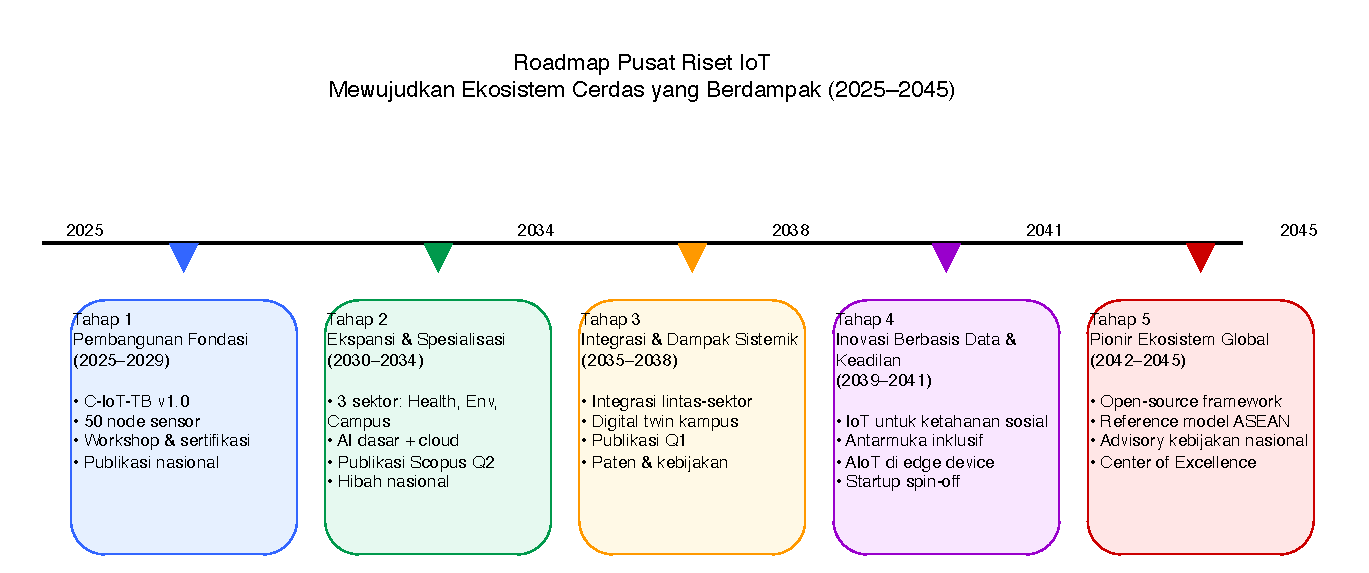
\includegraphics[width=\textwidth]{roadmapdiagram.pdf}
    \caption{Roadmap Strategis Pusat Riset IoT 2025–2045}
    \label{fig:roadmap}
\end{figure}

% \begin{center}
% \begin{tabular}{ll}
% \toprule
% \textbf{Indikator Keberhasilan} & \textbf{Target (Tahun 2045)} \\
% \midrule
% C-IoT-TB menjadi open-source reference model & Diakui di GitHub ($\geq$ 500 stars) \\
% Dipakai oleh $\geq$ 5 institusi lain (di Indonesia \& ASEAN) & Ada \\
% Publikasi di jurnal Q1 top-tier (Nature Digital Health, IEEE IoT Journal) & $\geq$ 15 \\
% Grup dipercaya sebagai advisory body pemerintah untuk kebijakan IoT & Ada \\
% Alumni memimpin departemen IoT di universitas/industri ternama & $\geq$ 5 \\
% Grup menjadi center of excellence di level ASEAN & Diakui oleh ASEAN IoT Council \\
% Visi awal terwujud: “Intelligent, interconnected ecosystem enhancing human well-being...” & Terukur \& diakui \\
% \bottomrule
% \end{tabular}
% \end{center}

% \begin{sidewaystable}
% \centering
% \caption{Indikator Keberhasilan Akhir Roadmap Riset IoT (Tahun 2045)}
% \label{tab:final-kpi}
% \begin{tabular}{lp{8cm}}
% \toprule
% \textbf{Indikator Keberhasilan} & \textbf{Target (Tahun 2045)} \\
% \midrule
% C-IoT-TB menjadi open-source reference model & Diakui di GitHub ($\geq$ 500 stars), dengan dokumentasi lengkap, contoh kasus implementasi, dan komunitas aktif pengembang. \\
% Dipakai oleh $\geq$ 5 institusi lain (di Indonesia \& ASEAN) & Setidaknya 5 universitas/instansi pemerintah di Indonesia dan ASEAN telah mengadopsi arsitektur C-IoT-TB sebagai fondasi proyek IoT mereka, dengan dokumentasi kerja sama resmi. \\
% Publikasi di jurnal Q1 top-tier (Nature Digital Health, IEEE IoT Journal, etc.) & Minimal 15 artikel ilmiah di jurnal Q1 Scopus/WoS, dengan fokus pada inovasi IoT berkeadilan, AIoT edge, atau dampak sosial teknologi. \\
% Grup dipercaya sebagai advisory body pemerintah untuk kebijakan IoT & Terlibat secara formal dalam penyusunan rekomendasi kebijakan nasional IoT oleh Kemenkominfo, BRIN, atau lembaga setara. \\
% Alumni memimpin departemen IoT di universitas/industri ternama & Minimal 5 alumni menjadi kepala laboratorium, dosen senior, atau manajer teknologi di universitas bergengsi (UI, ITB, UGM) atau perusahaan teknologi global (Huawei, Siemens, Telkomsel Digital). \\
% Grup menjadi center of excellence di level ASEAN & Diakui secara resmi oleh ASEAN IoT Council atau badan setara sebagai pusat unggulan riset IoT berkelanjutan dan berkeadilan di kawasan Asia Tenggara. \\
% Visi awal terwujud: “Intelligent, interconnected ecosystem enhancing human well-being, sustainability, and resilience” & Terukur melalui studi dampak independen (misal: oleh LKPP atau universitas mitra), yang menunjukkan peningkatan nyata pada kesejahteraan, keberlanjutan, atau ketahanan di 3 sektor utama (kesehatan, lingkungan, smart campus). \\
% \bottomrule
% \end{tabular}
% \end{sidewaystable}

\begin{sidewaystable}
    \centering
    \caption{Indikator Keberhasilan Akhir Roadmap Riset IoT (Tahun 2045)}
    \label{tab:final-kpi}
    \footnotesize % <<< Font sangat kecil, tapi masih terbaca
    \setlength{\tabcolsep}{3pt} % <<< Kurangi jarak antar kolom
    \renewcommand{\arraystretch}{0.9} % <<< Perkecil tinggi baris
    \begin{tabular}{lp{7.5cm}}
        \toprule
        \textbf{Indikator Keberhasilan}                                                                                        & \textbf{Target (Tahun 2045)}                                                                                                                                   \\
        \midrule
        C-IoT-TB menjadi open-source reference model                                                                           & Diakui di GitHub ($\geq$ 500 stars), dengan dokumentasi lengkap, contoh implementasi, dan komunitas aktif.                                                     \\
        Dipakai oleh $\geq$ 5 institusi lain (di Indonesia \& ASEAN)                                                           & Setidaknya 5 universitas/instansi pemerintah mengadopsi arsitektur C-IoT-TB sebagai fondasi proyek IoT mereka, dengan dokumen kerja sama resmi.                \\
        Publikasi di jurnal Q1 top-tier (Nature Digital Health, IEEE IoT Journal, dll.)                                        & Minimal 15 artikel di jurnal Q1 Scopus/WoS, fokus pada IoT berkeadilan, AIoT edge, atau dampak sosial teknologi.                                               \\
        Grup dipercaya sebagai advisory body pemerintah untuk kebijakan IoT                                                    & Terlibat formal dalam penyusunan rekomendasi kebijakan nasional IoT oleh Kemenkominfo, BRIN, atau lembaga setara.                                              \\
        Alumni memimpin departemen IoT di universitas/industri ternama                                                         & Minimal 5 alumni menjadi kepala laboratorium, dosen senior, atau manajer teknologi di UI/ITB/UGM, Huawei, Telkomsel Digital, atau Siemens.                     \\
        Grup menjadi center of excellence di level ASEAN                                                                       & Diakui resmi oleh ASEAN IoT Council atau badan setara sebagai pusat unggulan riset IoT berkelanjutan dan berkeadilan di Asia Tenggara.                         \\
        Visi awal terwujud: “Intelligent, interconnected ecosystem enhancing human well-being, sustainability, and resilience” & Terukur melalui studi dampak independen (misal: LKPP/universitas mitra), menunjukkan peningkatan nyata di 3 sektor utama: kesehatan, lingkungan, smart campus. \\
        \bottomrule
    \end{tabular}
\end{sidewaystable}

\textbf{Target Akhir:} Grup menjadi \textbf{pionir global dalam ekosistem IoT yang berkelanjutan dan adil}.

\section{Strategi Penting untuk Keberhasilan}

\begin{enumerate}
    \item \textbf{Start Small, Think Big}: Jangan tunggu dana besar — mulai dari 1 sensor, 1 ruangan, 1 masalah nyata.
    \item \textbf{Build Community, Not Just Tech}: Libatkan mahasiswa, staf, petugas kebersihan, lansia — mereka adalah pengguna akhir.
    \item \textbf{Openness is Power}: Publikasikan semua data, kode, desain. Ini akan menarik kolaborator dan dana.
    \item \textbf{Ethics First}: Jangan biarkan teknologi mengabaikan privasi, kesetaraan, atau kerentanan.
    \item \textbf{Celebrate Every Milestone}: Bahkan satu sensor yang berfungsi sudah merupakan kemajuan. Motivasi = momentum.
\end{enumerate}

\section{Kolaborasi \& Ekosistem}
\begin{enumerate}
    \item Akademik: riset bersama, pengembangan kurikulum IoT.
    \item Industri: joint research, kebutuhan pasar, prototyping.
    \item Pemerintah: regulasi, pendanaan, kebijakan smart city/smart farming.
    \item Komunitas \& Startup: inkubasi, hackathon, kompetisi.
\end{enumerate}
Untuk mewujudkan ekosistem IoT yang berdampak secara sistemik, kolaborasi multidimensi bukan sekadar pilihan, melainkan kebutuhan strategis. Sinergi antara akademik, industri, pemerintah, dan komunitas lokal membentuk siklus inovasi yang berkelanjutan: perguruan tinggi menjadi pusat riset dan pengembangan kapasitas SDM, industri memberikan tantangan nyata dan akses ke pasar, pemerintah menyediakan regulasi pendukung serta skala implementasi, sementara komunitas dan startup berperan sebagai agen perubahan di lapangan yang membawa teknologi ke ujung tombak layanan publik. Dengan membangun mekanisme kemitraan formal—seperti laboratorium bersama, program magang terstruktur, inkubator riset terapan, dan forum kebijakan berbasis bukti—grup ini tidak hanya menciptakan solusi teknis, tetapi juga membangun jaringan sosial-tekno yang mampu menjaga keberlanjutan, replikabilitas, dan skalabilitas inovasi. Dalam konteks Indonesia, pendekatan ini sekaligus menjawab tantangan kesenjangan digital dan mendorong transformasi dari technology adoption menuju technology ownership, sehingga IoT bukan lagi eksklusif milik institusi besar, melainkan menjadi alat pemberdayaan kolektif yang dipimpin oleh akademik lokal.

\section{Output \& Dampak}
\begin{enumerate}
    \item Produk riset: publikasi, paten, prototipe.
    \item Teknologi siap pakai: perangkat, aplikasi, platform.
    \item Kebijakan \& standar: rekomendasi untuk pemerintah/industri.
    \item SDM unggul: dosen, mahasiswa, peneliti berkompetensi IoT.
    \item Ekonomi \& sosial: inovasi yang mendukung UMKM, layanan publik, efisiensi industri.
\end{enumerate}

Output dari Pusat Riset IoT Polinema tidak hanya diukur oleh jumlah publikasi atau prototipe teknis, tetapi oleh dampak sistemik yang terwujud dalam ekosistem nyata. Setiap produk riset — mulai dari jurnal ilmiah hingga perangkat IoT yang diimplementasikan di kampus atau komunitas — dirancang sebagai pilar transformasi: publikasi membangun legitimasi akademik, paten melindungi inovasi lokal, dan prototipe menjadi bukti konsep yang dapat direplikasi; teknologi siap pakai menjembatani kesenjangan antara laboratorium dan lapangan; rekomendasi kebijakan mendorong adopsi berbasis bukti di tingkat pemerintah; SDM unggul menjadi agen perubahan yang menyebarluaskan kapasitas ke institusi lain; sementara dampak ekonomi dan sosial membuktikan bahwa IoT bukan sekadar teknologi canggih, melainkan alat pemberdayaan yang meningkatkan efisiensi layanan publik, memperkuat ketahanan UMKM, dan mengurangi kesenjangan digital. Dengan demikian, pusat ini bergerak dari research for knowledge menuju research for impact, secara konsisten menjawab tuntutan Kemendikbudristek untuk menciptakan riset yang relevan, berkelanjutan, dan bermanfaat bagi masyarakat luas.

% \section{Tim Perumus}
% Indrazno Siradjuddin, Erfan Rohadi, Devi Mega Risdiana, Rakhmat Arianto, Vipkas Al Hadid Firdaus, Rudy Ariyanto, Ahmadi Yuli Ananta, Ade Ismail, Usman Nurhasan.
\newpage

% \section{Tim Perumus}

% Dokumen Roadmap Pusat Riset IoT Polinema ini ditetapkan pada:

% \begin{center}
% \textbf{Politeknik Negeri Malang} \\
% \textit{Malang, 5 April 2025} \\
% \end{center}

% \noindent
% Dengan ini, tim perumus menyatakan bahwa dokumen ini merupakan hasil konsensus dan kontribusi intelektual seluruh anggota, serta menyetujui isi dan arah strategisnya.

% \vspace{1.5cm}

% \begin{tabular}{|p{5cm}|p{8cm}|}
% \hline
% \textbf{Nama} & \textbf{Tanda Tangan} \\ 
% \hline
% Indrazno Siradjuddin & \hspace{5cm} \\
% \hline
% Erfan Rohadi & \hspace{5cm} \\
% \hline
% Devi Mega Risdiana & \hspace{5cm} \\
% \hline
% Rakhmat Arianto & \hspace{5cm} \\
% \hline
% Vipkas Al Hadid Firdaus & \hspace{5cm} \\
% \hline
% Rudy Ariyanto & \hspace{5cm} \\
% \hline
% Ahmadi Yuli Ananta & \hspace{5cm} \\
% \hline
% Ade Ismail & \hspace{5cm} \\
% \hline
% Usman Nurhasan & \hspace{5cm} \\
% \hline
% \end{tabular}

% \vspace{1cm}
% \noindent
% \textit{Catatan: Dokumen ini sah apabila telah ditandatangani oleh seluruh anggota tim perumus dan dilegalisasi oleh pimpinan institusi.}

\section{Tim Perumus}

Dokumen Roadmap Pusat Riset IoT Polinema ini ditetapkan pada:

\begin{center}
    \textbf{Politeknik Negeri Malang} \\
    \textit{Malang, 12 September 2025} \\
\end{center}

\noindent
Dengan ini, tim perumus menyatakan bahwa dokumen ini merupakan hasil konsensus dan kontribusi intelektual seluruh anggota, serta menyetujui isi dan arah strategisnya.

\vspace{2.2cm} % Spasi sebelum tabel

\begin{tabular}{|p{5cm}|p{8cm}|}
    \hline
    \textbf{Nama}           & \textbf{Tanda Tangan} \\
    \hline
    Indrazno Siradjuddin    &                       \\[1.2cm] % Ruang tanda tangan lebih tinggi
    \hline
    Erfan Rohadi            &                       \\[1.2cm]
    \hline
    Devi Mega Risdiana      &                       \\[1.2cm]
    \hline
    Rakhmat Arianto         &                       \\[1.2cm]
    \hline
    Vipkas Al Hadid Firdaus &                       \\[1.2cm]
    \hline
    Rudy Ariyanto           &                       \\[1.2cm]
    \hline
    Ahmadi Yuli Ananta      &                       \\[1.2cm]
    \hline
    Ade Ismail              &                       \\[1.2cm]
    \hline
    Usman Nurhasan          &                       \\[1.2cm]
    \hline
\end{tabular}

\vspace{2cm} % Spasi setelah tabel

% \noindent
% \textit{Catatan: Dokumen ini sah apabila telah ditandatangani oleh seluruh anggota tim perumus dan dilegalisasi oleh pimpinan institusi.}


\newpage

\section{Penutup}

Roadmap ini memberikan jalan realistis bagi pusat riset IoT yang baru dimulai dari nol. Dengan konsistensi, keberanian untuk belajar, dan komitmen terhadap nilai kemanusiaan dan keberlanjutan, tim ini tidak hanya akan bertahan — tetapi akan menjadi \textbf{kekuatan transformasional} dalam ekosistem IoT nasional dan global.

\textit{“Anda tidak perlu menjadi ahli IoT hari ini — Anda hanya perlu memulai hari ini, dan terus belajar setiap minggu.”}



\end{document}